\refstepcounter{chapter}
\chapter{Image Processing}



Computational Photography

Bayer Pattern

Camera noise models

\subsection{Integral Images}


The value at any point (*x*, *y*) in the summed-area table is the sum of all the pixels above and to the left of (*x*, *y*), inclusive where $i(x,y)$  is the value of the pixel at (x,y). The summed-area table can be computed efficiently in a single pass over the image:

$I(x,y) = i(x-1,y-1) + I(x,y-1) + I(x-1,y)-I(x-1,y-1)$

and similarly for any rectangular region:

$ i(A,B,c,D) = I(D) - I(B) - I(C)+I(A)$

\includegraphics{https://upload.wikimedia.org/wikipedia/commons/thumb/5/58/Summed_area_table.png/220px-Summed_area_table.png}

\section{ Filtering}
\begin{itemize}
\item Color Conversion
\item Thresholding
\item Smoothing
\item Morphology
\item Gradients
\item Canny Edge Detection
\item Contours
\item Histograms
\end{itemize}

\subsection{Convolution}

\subsection{Denoising}

Median/mean filtering

\subsection{Deblurring}

\subsubsection{Fourier Transform}

\subsection{Pattern / Function Matching }

\subsection{Gaussian Pyramids}



Gradient consistency assumption + intensity consistency assumption

Iterative multi scale + warping

Uses an analytic formulation derived from Euler-Lagrange Equations

Results in a dense optic flow field.

Works well for small changes.

\section{Up and Down Sampling}


Nearest Neighbor

Linear

Bi-linear

\section{Noise Models}

\subsubsection{Salt and Pepper / Black White}

This type of noise happens due to sudden interruption in the image signal.

Can be removed using median or morphological filtering.

\subsubsection{Gaussian noise}

\subsubsection{Blue noise}

\section{Semantic Computer Vision} 

Visual Odometry

\subsubsection{Silhouette Segmentation / Visual Hull}

\section{Optic Flow}


\section{Image Segmentation / Pixel Labeling}

\section{Object Detection}

\section{Classification Problems}


\section{Event Cameras}

\subsubsection{Features}

\begin{itemize}
\item Low-latency (~ 1 μs)
\item No motion blur
\item High dynamic range (140 dB instead of 60 dB)
\item Ultra-low power (mean: 1mW vs 1W)
\end{itemize}

Traditional vision algorithms cannot be used because:
\begin{itemize}
\item Asynchronous pixels
\item No intensity information (only binary intensity changes)
\end{itemize}

But they bring new possibilities:
\begin{itemize}
\item Night vision
\item Compact representation and data
\end{itemize}

On static scenes, they mostly produce noise

Main visible features - edges. 

\subsubsection{Linearized Event Generation}

An event is triggered $\log I(x,t) \log I(xt-\Delta t)=\pm C$

Where $C$ 

Consider a pixel $p(x,y)$ with gradient $\nabla L(x,y)$ undergoing a motion $u\in(u,v)$ induced by a moving point $p \in\mathbb{R}^3 $

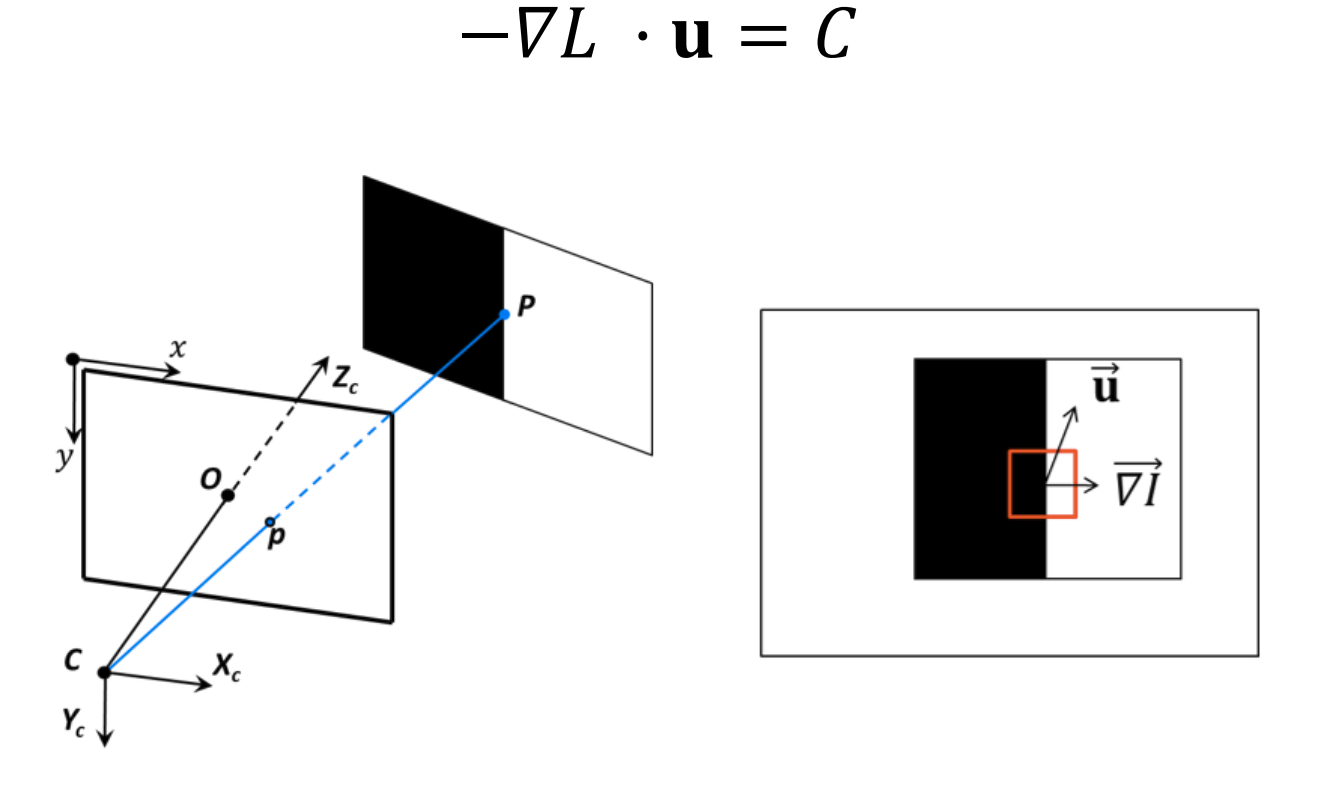
\includegraphics{event_cameras_fig/event_cameras.png}

From brightness constancy assumption:

$L(x,y,t) = L(x+u,y+v,t+\Delta t)$ from first order approx we get the following $-\nabla L \cdot \vec u = C$

\subsubsection{Deblurring}

A blurry image can be regarded as the integral of a sequence of latent images during the exposure time, while the events indicate the changes between the latent images.

Sharp images are done by subtracting the double integral of the events

\subsubsection{(Sparse) Feature Tracking In Event Space}

\subsubsection{Kanade–Lucas–Tomasi}

Goal: extract features on frames and track them using only events in the blind time between two frames

Uses the event generation model via joint estimation of patch warping and optic flow

Disadvantages: requires GPU for real time tracking and they require knowledge of contract sensitivity, which is scene dependent and differs from pixel to pixel.	

\subsubsection{Image Reconstruction from Event Cameras}

Recurrent neural network (main module: Unet) 

Input: last reconstructed frame + sequences of event tensors (spatiotemporal 3D voxels grid: each voxel contains sum of ON and OFF events falling within the voxel)

Network processes last $N$ events (10,000) 

Trained in simulation only (without seeing a single real image) (we used our event camera simulator: http://rpg.ifi.uzh.ch/esim.html) 

Noise free simulation. We randomized the contrast sensitivity

